\documentclass[a4paper, titlepage]{article}
\usepackage[T1]{fontenc}
\usepackage[swedish]{babel}
\usepackage[utf8]{inputenc}
\usepackage{graphicx}
\usepackage[normalem]{ulem}
\title{
    Programming Project \\
    C++ Programming(EDA031)
}
\author{
        Department of Computer Science \\
            \\
        Simon Thörnqvist (ada09st1@student.lth.se)
            \and
        Fredrik Pettersson (ada09fpe@student.lth.se)
            \and
        Marcus LindFeldt (ada08mli@student.lth.se)
            \and
        [Robobuilder enter name and email here]
}
\date{\today}
\begin{document}
\maketitle

\section{Introduction}\label{introduction}
The purpose of this project was to implement a news system similar to the Usenet News. The assignment included the implementation of the server, the client and the communication between them. NNTP was the protocol used for the communication.
 
\section{Requirements}\label{requirements}

\section{System Outline}\label{systemoutline}
\subsection{Com}

\subsection{Database}

\subsection{Server}

\subsection{Client}

\section{Summary}\label{summary}

\newpage
\appendix
\section{UML Diagram}\label{App:AppendixA}
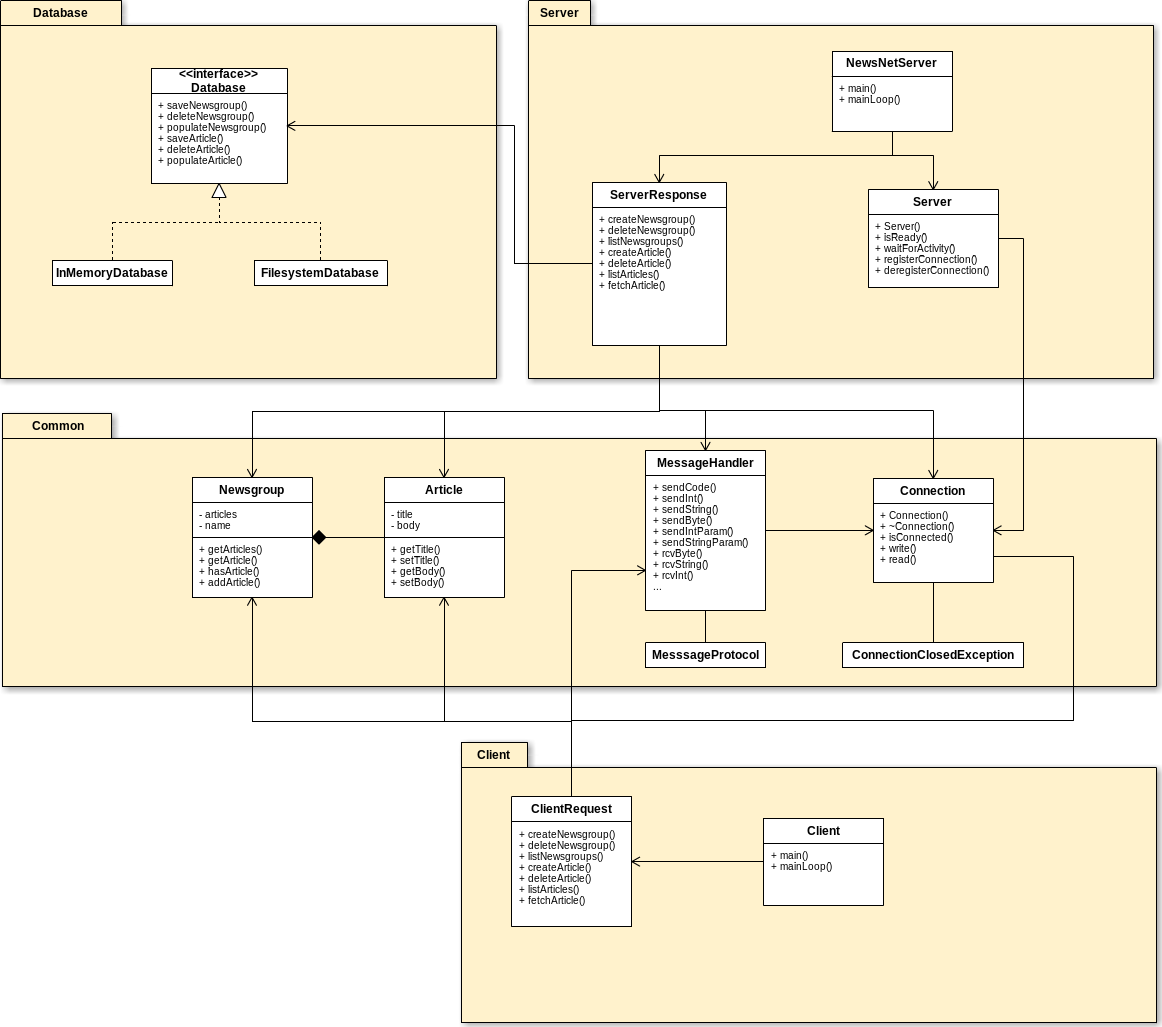
\includegraphics[width=130mm]{NewsNet_UML.png}

\end{document}